\documentclass[11pt, a4paper]{report}
\usepackage[utf8]{inputenc}

\usepackage{listings}
\usepackage[framed,numbered,autolinebreaks,useliterate]{mcode}

\usepackage[margin=1in]{geometry}
\usepackage{graphicx}
\usepackage{amsmath}
\usepackage{amsfonts}
\usepackage{caption}
\usepackage{float}
\usepackage{hyperref}
\usepackage{appendix}
\usepackage{chngcntr}
\usepackage{etoolbox}
\usepackage{lipsum}
\usepackage{tikz}
\graphicspath{ {images/} }
\setlength\parindent{0pt}


\newcommand{\p}{\partial}
\newcommand{\mth}[1]{
  \begin{align*}
    #1
  \end{align*}
}


\usetikzlibrary{shapes.geometric, arrows}

\newcommand{\newappendix}{%
  \refstepcounter{chapter}\chapter*{Appendix \thechapter}%
  \addcontentsline{toc}{chapter}{Appendix \thechapter}%
}
\tikzstyle{block} = [rectangle, rounded corners, minimum width=3cm, minimum height=1cm,text centered, draw=black, fill=white!30]
\tikzstyle{startstop} = [rectangle, rounded corners, minimum width=3cm, minimum height=1cm,text centered, draw=black, fill=red!30]
\tikzstyle{io} = [trapezium, trapezium left angle=70, trapezium right angle=110, minimum width=3cm, minimum height=1cm, text centered, draw=black, fill=blue!30]
\tikzstyle{process} = [rectangle, minimum width=3cm, minimum height=1cm, text centered, draw=black, fill=orange!30]
\tikzstyle{decision} = [diamond, minimum width=3cm, minimum height=1cm, text centered, draw=black, fill=green!30]
\tikzstyle{arrow} = [thick,->,>=stealth]

\begin{document}

\begin{center}
  \Huge Floppy Drive Orchestra \\
  \huge University of Colorado Boulder \\
  \Large Independent Study 2017\\
  
  \vspace{6in}
    \huge Jeffery Lim \\
    \huge Jeffery.Lim@colorado.edu\\
    \Large Under supervision of Dr. Shalom Ruben \\~\\~\\
\end{center}

\tableofcontents

\chapter{Introduction}

The goal of the floppy drive orchestra is to both develop a working orchestra with several floppy drives and to understand what allows the floppy drive orchestra function properly. Floppy drives are a hardware device invented in 1967 that was used to read and write information. THese floppy drives are now considered antique in the computer hardware world, and there is not much functionality to these drives. Several people, however, have abused the floppy drive to try and produce music from them, and thus, the floppy drive orchestra was born. \\

To understand the floppy drives, several tests were conducted to test their power consumption, physical limitation of the read/write head, and what ranges of frequencies does it play. The hardware to enable several floppy drives is explored, as well as the hardware on the Arduino. The MIDI, or musical instrument digital interface, is a special format that gives lots of information. Finally, the software to play music, as well as the software on the Arduino will be explored. 

\chapter{Floppy Drive Characteristics}

The first tests conducted were the analysis of a single floppy drive unit. Floppy drives come in three sizes: 8 in., 5.25 in., and 3.5 in. The large floppy drives come with different characteristics, however, the more modern 3.5 in. floppy drive will be used in this orchestra. The five characteristics to be explored are pinouts, power, stepper motor movements, stepper motor bandwidth, and frequency.

\begin{figure}[H]
\hspace*{-2cm}    
    \centering
    \includegraphics[width=.5\textwidth]{floppydrive_sizes.jpg}
    \caption{Floppy Drive of All Sizes}
    \label{fig:sizes}
\end{figure}


\section{Floppy Pinout}

The floppy pinout is shown in Figure \ref{fig:pinOut}. The bottom row, or the odd valued pins, are all grounded, where the top pins, or the even valued pins, are live. Each pin has a diferent functionality when it is grounded with the pins below. It is not necessary to connect the live pins to their respected ground pins, because the bottom row are all grounded. The actual names of the active pins are shown in Figure \ref{fig:pinNames}.

\begin{figure}[H]
\hspace*{-2cm}    
    \centering
    \includegraphics[width=.75\textwidth]{floppy_pinout.jpg}
    \caption{Floppy Drive Pinout}
    \label{fig:pinOut}
\end{figure}

\begin{figure}[H]
\hspace*{-2cm}    
    \centering
    \includegraphics[width=.75\textwidth]{pinNames.png}
    \caption{Floppy Drive Pin Names}
    \label{fig:pinNames}
\end{figure}

The only necessary pins to drive the floppy drive are pin number 12 or 14, 18, and 20. Pins 12 and 14 are the drive select B and A repectively. These are the drive enable pins. Some drives are B drives and others are A. In order to see the drive letter, connect pin 12 or 14 to one of the pin bottom pins: the LED will turn on for one drive letter. These pins are equivalent to an enable pin.\\

Pin 18 is a direction pin. The direction is what determines the direction of the motor drive. When the pin is grounded, the drive heads moves away from the pins, and when the pin is high, the drive returns towards the pins. \\

Pin 20 is a step pin. This pin drives the stepper motor. Every time the pin goes high, the stepper motor will go forward one tick.\\


\begin{figure}[H]
\hspace*{-2cm}    
    \centering
    \includegraphics[width=.75\textwidth]{floppy_pinoutV1.jpg}
    \caption{Floppy Drive Necessary Pins}
    \label{fig:pins}
\end{figure}

\section{Power}

The floppy drive takes a mini Molex cable as seen in Figure \ref{fig:miniMolex}. A mini Molex cable has 4 different lines, one red, one yellow, and two black. The two black wires are grounded, where the red line is 5V and the yellow is 12V. Older generation floppy drives used both the 5V and 12V, where the 12V was used to power the stepper motor. The modern floppy drives no longer use the 12V for stepper motors, and only use 5V. For the final floppy drive hardware, this results in only needing a 5V rail to power all of the floppy drives.

\begin{figure}[H]
\hspace*{-2cm}    
    \centering
    \includegraphics[width=.4\textwidth]{miniMolex.jpg}
    \caption{Floppy Drive Power Pinout}
    \label{fig:miniMolex}
\end{figure}


The power consumption was measured by using jumper cables to connect the floppy drives to a power supply, through an ammeter. Pin 12 is grounded, to enable drive B. When the drive is not running, the ammeter measured 50 mA. To test when active, pin 20 is connected to a function generator, generating a square wave. Pin 18 is grounded and set to high appropriately in order to allow the stepper motor to switch back and forth. When active, the floppy drive pulls 400 mA. The function generator was swept from all frequencies in order to see if a change in frequency would affect the current consumption, however, no change was made. This means that at most, each floppy drive requires around 400 mA. \\

\section{Stepper Motor Movement}

\begin{figure}[H]
\hspace*{-2cm}    
    \centering
    \includegraphics[width=.3\textwidth]{floppydrive_coveroff.jpg}
    \caption{Floppy Drive With Top Off}
    \label{fig:coveroff}
\end{figure}

The floppy drive read/write head has a physical limit to how far it can go. To determine this value, a 1 Hz square wave is sent through to the floppy drive's direction pin (pin 18). Pin 12 is grounded, and pin 18 is set to ground. The number of ticks is manually recorded by counting the number of audible ticks that can be heard, with the last value is when the read/write head does not move. This can be run multiple times by simply disconnected or connecting the direction pin, or pin 18. \\

The total number of ticks a 3.5 in. drive can go is 80, meaning the step pin (pin 20) needs to be toggled high 80 times before the drive reaches the limit. This means there needs to be a transition of high to low 80 times, or a total of 160 voltage transitions. Depending on the floppy drive, the motor will react differently when the read/write head reaches its limit. The head will either try and move, causing an audible ticking, while others will not move. \\

\section{Stepper Motor Bandwidth}

Since the music will be played through the read/write head, the bandwidth of the stepper motor will be a large limiting factor. For the test, a square wave from a waveform generator is connected to the step pin (pin 20), and the direction pin is connected to ground and disconnected in order to allow the read/write head to switch direction. \\

The waveform generator is swept from 1 Hz up until the read/write head is no longer moving. The drive was able to handle up to 400 Hz, but afterwards, it was no longer consistent in terms of the speed of the drive. This test is ran again when the software was fully written. This made a significant difference because the motor was able to run at a much higher input frequency. \\

This limit considerably restricts what the drive can play, and higher notes will need to be addressed. However, so far, there is an assumption that the audible range contains the input frequency given to the stepper motor. In the next section, audio files of the floppy drives at each frequency are recorded and transformed. \\

\section{Frequency}

Although the floppy drive was unable to run past 400 Hz, it is also important to take a look at the actual audio produced from the floppy drive. 


\chapter{Hardware}

In this chapter, the hardware setup of the orchestra is built. The microcontroller chosen for this project was an Arduino. The use of shields allow building a floppy drive orchestra much simpler. 

\section{Power}


As discussed in the previous chapter on floppy drive power characteristics, since each floppy drive, when running, draws 400 mA. For each floppy drive added to the system, the total power draw increases by 400 mA, so for 4 floppy drives, the total power consumption from the floppy drive system would be around 1600 mA, or 1.6 A. This means the power supply would need to be at least 2 A to take into consideration of the Arduino power consumption. This extra 400 mA would be plenty of enough to power the Arduino and run very extensive code. \\

The power is supplied from a 5V 2A power supply. This is directly connected into a power terminal. \\
  
\section{Cables}
All the wires bought were from Pololu, which can be found in Table \ref{fig:BOM}. \\

To build the wires, pre-crimped terminal wires were used. All wires bought were female wires. The power cord is simply a red and black wire connected to a 1 x 2 pin housing. 

The data cables were a little bit more complicated. The floppy drive pins had a 2 x 10 pin housing. This housing would be connected to the far left side of the floppy drive pins. The only pins connected are the same as seen in Figure \ref{pins}. Pins 11 and 12 are connected to black pre-crimped terminals. Pin 18 is connected to a blue pre-crimped terminal and pin 20 is connected to a purple pre-crimped terminal. Since pin 11 is grounded, there is no need for any other ground pins to come out. \\

On the other end of the data cable is a 2 x 2 pin housing. The order is significant and must be followed exactly. The two black wires can be connected to any pins, as long as they are on the same side. The blue and purple pin need to be in the following order: blue on the left, and purple on the right. This needs to be consistent because all of the direction pins are on even numbered pins and the step pins are on odd numbered pins. \\

\section{Schematic}

The following is the schematic of the shield. The shield purchased can be found in Table \ref{fig:BOM}. There are many ways to wire the shield, however, the easiest method is the following. 

With the shield, solder on all the components that come with the shield. Once finished, then following the layout of the shield as seen in Figure \ref{fig:TOP}.


\begin{figure}[H]
\hspace*{-2cm}    
    \centering
    \includegraphics[width=.3\textwidth]{TOP.jpg}
    \caption{Top of the Shield}
    \label{fig:TOP}
\end{figure}


\begin{figure}[H]
\hspace*{-2cm}    
    \centering
    \includegraphics[width=.3\textwidth]{TOP1.jpg}
    \caption{Top of the Shield}
    \label{fig:TOP1}
\end{figure}

\begin{figure}[H]
\hspace*{-2cm}    
    \centering
    \includegraphics[width=.3\textwidth]{TOP2.jpg}
    \caption{Top of the Shield}
    \label{fig:TOP2}
\end{figure}

On the bottom, ensure that the wires are hooked accordingly. The grounded wires are colored black, while the 5V lines are colored red.

\begin{figure}[H]
\hspace*{-2cm}    
    \centering
    \includegraphics[width=.3\textwidth]{BOT.jpg}
    \caption{Bottom of the Shield}
    \label{fig:BOT}
\end{figure}



\chapter{MIDI Files}

MIDI, or Musical Instrument Digital Interface, is a standard that has its own protocols, interface, and connectors. It allows a single file to contain multiple tracks for several instruments in its own channel. This allows a MIDI file to play several instruments at once, up to a maximum of 16 instruments. This advantage of the MIDI file allows multiple floppy drives to be played at once, like how a MIDI file would normally send notes to several instruments. 

\section{MIDI Notes}

The MIDI interface has notes that are mapped to specific piano keys at their respected frequencies. Each note is represented by a byte, or 8 bits, however, it does not use the top bit, meaning the notes go from 0 to 127. In Figure \ref{fig:Piano}, the respected MIDI note number has an associated piano key, since the MIDI note is based on music pitch. In Table \ref{fig:note2freq}, the actual frequency of the MIDI note number is displayed in hertz. Because of the earlier findings on the floppy drive characteristics, there are a lot of notes that may not be played. Assuming the floppy drive limit is 400 Hz, notes 0 to 67, or at least half of the range can be played. 

\begin{figure}[H]
\hspace*{-2cm}    
    \centering
    \includegraphics[width=.75\textwidth]{midi_notechart.jpg}
    \caption{MIDI Note Number to Piano Key}
    \label{fig:Piano}
\end{figure}


\captionof{table}{MIDI Note to Frequency}\label{fig:note2freq}
\begin{center}
 \begin{tabular}{|c|c||c|c||c|c||c|c|} 
 \hline
 MIDI Note& Hz & MIDI Note& Hz & MIDI Note& Hz & MIDI Note&Hz\\
 \hline
 0 & 8.18 & 32 & 51.91& 64 & 329.63 & 96 & 2093.00 \\
 \hline
1 & 8.66 & 33 & 55.00& 65 & 349.23 & 97 & 2217.46 \\
 \hline
2 & 9.18 & 34 & 58.27& 66 & 369.99 & 98 & 2349.32 \\
 \hline
3 & 9.72 & 35 & 61.74& 67 & 392.00 & 99 & 2489.02 \\
 \hline
4 & 10.30 & 36 & 65.41& 68 & 415.30 & 100 & 2637.02 \\
 \hline
5 & 10.91 & 37 & 69.30& 69 & 440.00 & 101 & 2793.83 \\
 \hline
6 & 11.56 & 38 & 73.42& 70 & 466.16 & 102 & 2959.96 \\
 \hline
7 & 12.25 & 39 & 77.78& 71 & 493.88 & 103 & 3135.96 \\
 \hline
8 & 12.98 & 40 & 82.41& 72 & 523.25 & 104 & 3322.44 \\
 \hline
9 & 13.75 & 41 & 87.31& 73 & 554.37 & 105 & 3520.00 \\
 \hline
10 & 14.57 & 42 & 92.50& 74 & 587.33 & 106 & 3729.31 \\
 \hline
11 & 15.43 & 43 & 98.00& 75 & 622.25 & 107 & 3951.07 \\
 \hline
12 & 16.35 & 44 & 103.83& 76 & 659.26 & 108 & 4186.01 \\
 \hline
13 & 17.32 & 45 & 110.00& 77 & 698.46 & 109 & 4434.92 \\
 \hline
14 & 18.35 & 46 & 116.54& 78 & 739.99 & 110 & 4698.64 \\
 \hline
15 & 19.45 & 47 & 123.47& 79 & 783.99 & 111 & 4978.03 \\
 \hline
16 & 20.60 & 48 & 130.81& 80 & 830.61 & 112 & 5274.04 \\
 \hline
17 & 21.83 & 49 & 138.59& 81 & 880.00 & 113 & 5587.65 \\
 \hline
18 & 23.12 & 50 & 146.83& 82 & 932.33 & 114 & 5919.91 \\
 \hline
19 & 24.50 & 51 & 155.56& 83 & 987.77 & 115 & 6271.93 \\
 \hline
20 & 25.96 & 52 & 164.81& 84 & 1046.50 & 116 & 6644.88 \\
 \hline
21 & 27.50 & 53 & 174.61& 85 & 1108.73 & 117 & 7040.00 \\
 \hline
22 & 29.14 & 54 & 185.00& 86 & 1174.66 & 118 & 7458.62 \\
 \hline
23 & 30.87 & 55 & 196.00& 87 & 1244.51 & 119 & 7902.13 \\
 \hline
24 & 32.70 & 56 & 207.65& 88 & 1318.51 & 120 & 8372.02 \\
 \hline
25 & 34.65 & 57 & 220.00& 89 & 1396.91 & 121 & 8869.84 \\
 \hline
26 & 36.71 & 58 & 233.08& 90 & 1479.98 & 122 & 9397.27 \\
 \hline
27 & 38.89 & 59 & 246.94& 91 & 1567.98 & 123 & 9956.06 \\
 \hline
28 & 41.20 & 60 & 261.63& 92 & 1661.22 & 124 & 10548.08 \\
 \hline
29 & 43.65 & 61 & 277.18& 93 & 1760.00 & 125 & 11175.30 \\
 \hline
30 & 46.25 & 62 & 293.66& 94 & 1864.66 & 126 & 11839.82 \\
 \hline
31 & 49.00 & 63 & 311.13& 95 & 1975.53 & 127 &  12543.85 \\
 \hline
 \end{tabular}
\end{center}


\section{MIDI} \label{MIDIMESSAGE}

MIDI data is sent serially, meaning the data is sent one bit at a time. As a result, the Arduino will be accepting the data from a serial port. In order for the MIDI data to be understood, the messages sent need to be understood. MIDI files are separated into two parts: a header chunk and a track chunk. Each chunk is separated into three sections known as type of chunk, length of the data, and data. 

\subsection{Header Chunk}

The first 4 bytes are an ASCII representation of what type of chunk it is. This is always MThd for the header. The next 4 bytes is the length of the data section. The data section is a total of 6 bytes. The first 16 bits is the MIDI format. MIDI files comes in three formats: Format 0, Format 1, and Format 2. Format 0 is a single track format, where there is only one track or one instrument. Format 1 has multiple tracks, each to be played simultaneously. Format 2 has multiple tracks, each to be played independently. The next 16 bits are the number of tracks. The last 16 bits are the time divisions. There are two formats depending on the upper bit. \\


\captionof{table}{Header Chunk}\label{fig:header}
\begin{center}
 \begin{tabular}{||c | c | c | c | c||} 
 \hline
  \multicolumn{5}{|c|}{Header Chunk} \\ 
 \hline
  \multicolumn{3}{|c|}{Chunk Type}  & Length & Data \\
 \hline
  ASCII (4 Bytes) & Length of Data(4 Bytes)  & Format (16 bits) & Tracks (16 bits) & Division (16 bits) \\
 
 \hline
\end{tabular}
\end{center}

If the upper bit is 0, then the value represents the number of time ticks per quarter note. If the upper bit is 1, then bits 0 to 7 represent the number of delta-time units per SMTPE frame. Bits 8 to 14 form the number of SMTPE frames per second. \\

\subsection{Track Chunk}

The track chunk starts out the same as the header chunk. The first 4 bytes are the ASCII representation and is always MTrk. It then gives the length of data of the data section. The last section is the data, which contains delta times and events. There are three types of events, however, the one that will be focused on are the MIDI events.


\captionof{table}{Track Chunk}\label{fig:track}
\begin{center}
 \begin{tabular}{||c | c | c||} 
 \hline
  \multicolumn{3}{|c|}{Track Chunk} \\ 
 \hline
  Chunk Type & Length & Data \\
 \hline
  ASCII (4 Bytes) & Length of Data(32 bits)  &  Delta Time and Events \\
 
 \hline
\end{tabular}
\end{center}


\subsection{MIDI Message}

The events that the track chunk talks about are the MIDI messages that are important to playing notes. Each message comes in 3 bytes. The first byte are a status byte that contains a command and channel. There are several commands, but for the floppy drive orchestra, there is only two commands that are important: note on and note off. The channel bits are the MIDI channels that the message is suppose to go to. \\

The last two bytes are the note and velocity The velocity represents the loudness of the note. A zero velocity would have no sound, and anything above would mean to play the note. Since the floppy drive cannot produce a louder noise, we can effectively ignore it, unless it is equal to zero.

\captionof{table}{MIDI Message}\label{fig:midimessage}
\begin{center}
 \begin{tabular}{||c | c | c | c | c||} 
 \hline
  \multicolumn{5}{|c|}{MIDI Message} \\ 
 \hline\hline
  \multicolumn{3}{|c|}{Status}  & Data & Data \\
 \hline
  \multicolumn{2}{|c|} {Command (4 bits)} & Channel(4 bits)  & Note (8 bits) & Velocity (8 bits) \\
 \hline
  Note On & 1001 & nnnn  & 0xxxxxxx & 0vvvvvvv \\
 \hline  
  Note Off  & 1000 & nnnn  & 0xxxxxxx & 0vvvvvvv \\
 \hline
\end{tabular}
\end{center}

\subsection{Delta Time}

Delta time is the number of ticks needed until the next event. This is a crucial part of the data stream because it lets the instrument or player know that there needs to be waiting until the next note plays. This part is not important to running the floppy drive orchestra from the computer because the player will handle the ticks, however, if the Arduino is handling everything, it needs to keep track of the ticks.

\chapter{Software}

In order to run the software, there needs to be information to be sent from a computer to the Arduino. 

\section{Using a PC}

The data flow path of the driver is as following. 

\begin{center}
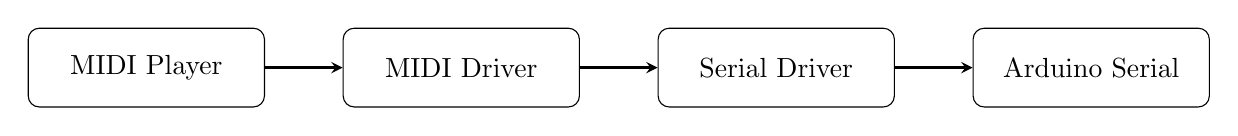
\begin{tikzpicture}[node distance=2cm]

\node (block) [block] {MIDI Player};
\node (block1) [block, right of=block, xshift=2cm] {MIDI Driver};
\node (block2) [block, right of=block1, xshift=2cm] {Serial Driver};
\node (block3) [block, right of=block2, xshift=2cm] {Arduino Serial};

\draw [arrow] (block) -- (block1);
\draw [arrow] (block1) -- (block2);
\draw [arrow] (block2) -- (block3);

\end{tikzpicture}
\end{center}


\subsection{MIDI to Serial Driver}

The MIDI to serial driver is a key player in getting music to play on the floppy drives. The driver turns the MIDI outputs from the player, into data that is transmitted using serial. The driver used for this project was Hairless MIDI to Serial Bridge, found at \cite{HairlessMIDI}. \\

This project has platforms for all three operating systems and has a GUI that is easy to interface with as evident in Figure \ref{fig:hairless}. The Serial<->MIDI Bridge On turns the driver on or off, being necessary with reprogramming the Arduino since the Arduino requires the serial port to be programmed. The Serial Port drop down menu will have the name of the Arduino or the COM port being used by the Arduino. The MIDI In drop down menu is where the MIDI player or piano should be located. \\


\begin{figure}[H]
\hspace*{-2cm}    
    \centering
    \includegraphics[width=.75\textwidth]{MIDISerial_Bridge.png}
    \caption{Hairless MIDISerial}
    \label{fig:hairless}
\end{figure} 

The second MIDI to Serial Driver that works on Linux is known as ttymidi. This is a MIDI to serial driver that does not have a GUI and is all done on the command line. It is significantly more difficult to install and understand.

\subsection{Virtual Keyboard}

There is a program called VMPK or Virtual MIDI Piano Keyboard that sends MIDI file based on the note played \cite{VMPK}. This is a great way of testing the MIDI parser on the Arduino and testing the floppy drive's responsiveness to different notes. It will work on Linux or Mac.  

The only necessary step is to go to EDIT -$>$ MIDI Connections and make sure that Enable MIDI input is selected as following:

\begin{figure}[H]
\hspace*{-2cm}    
    \centering
    \includegraphics[width=.75\textwidth]{HairlessSetup.png}
    \caption{Hairess MIDI Setup}
    \label{fig:hairlesssetup}
\end{figure} 

Once it is enabled, Hairless MIDI should show an option to set MIDI IN to VMPK. This will route the MIDI notes played from the piano to the Arduino. 

\subsection{MIDI Player}

The MIDI player is just like any audio player, with the exception of the ability to parse through the MIDI file format. There are specifications that must be met in order to use a MIDI player with the serial driver. The Hairless MIDI to Serial Bridge website, \cite{HairlessMIDI} does a good job of explaining further what needs to be done in order to work with MIDI players, but does not provide any programs that work with them. The MIDI player does some back-work for the Arduino: it handles the header and the delta time ticks. It sends the note on and note off messages at the correct time and keeps track of the beat. 

\subsubsection{Hairless MIDI}

In Linux, one must use ALSA, or advanced linux sound architecture. This architecture gives sound cards a good API with lots of features. The most important feature is the ability to work with MIDI. The two major programs necessary are pmidi, which can be downloaded at \cite{pmidi}, and aconnect, which is preinstalled on most flavors of Linux.

The first step is to know which port to send pmidi data through. The following command lists out the different ports available.

\begin{lstlisting}[language=bash]
  $ pmidi -l
   Port     Client name                       Port name
   14:0     Midi Through                      Midi Through Port-0
\end{lstlisting}

Midi Through Port-0 is the port needed to send MIDI data through. The next step is to go to Hairless MIDI and set the MIDI In to Midi Through Port-0. This connects serial to Midi Through Port-0. Any data sent to this port will be sent out to the USB Port. \\

The final step is to have pmidi play the music file. The command to do so is:


\begin{lstlisting}[language=bash]
  $ pmidi -p 14:0 [music file]
\end{lstlisting}

The -p signifies the port number, this case, 14:0, for Midi Through Port and the music file is the directory to the .mid file. \\


\subsection{ttymidi}

In order to use ttymidi, first download it from the link \cite{ttymidi}. Once it has been downloaded, ensure the system has libasound2, a library Used to work with ALSA. To install this library:


\begin{lstlisting}[language=bash]
  $ sudo apt-get install libasound2-dev
\end{lstlisting}

Next, edit the Makefile to add -lpthread to the line after all:

\begin{lstlisting}[language=bash]
all:
    gcc src/ttymidi.c -o ttymidi -lasound -lpthread
\end{lstlisting}

Once these steps have been taking, the next two commands will make the library and install it. 

\begin{lstlisting}[language=bash]
  $ make
  $ make install
\end{lstlisting}

In order to start ttymidi, ensure that the Arduino is plugged into the computer. It can be found in the dev directory and is usually named ttyACM0. 

\begin{lstlisting}[language=bash]
  $ ls /dev
\end{lstlisting}

Once you have figured out which directory it is, the next line initalizes the drivers.

\begin{lstlisting}[language=bash]
  $ ttymidi -s /dev/ttyACM0 -b 115200
\end{lstlisting}






\section{Arduino}

The code written for the project was done entirely in arduino.

\section{SD Card(?)}

\chapter{Arduino}

\section{Parameters}
There are several global parameters used in order to do the control of the floppy drives. Each parameter are arrays of a set size, set specifically to the number of floppy drives in the system. For example, array[0] would be for the first floppy drive, and array[1] would be for the second. 

\lstinputlisting[language=C, firstline=1, lastline=33]{../src/floppy/floppy.ino}

There are a couple of preset defines. NUMDRIVES is simply the number of drives the Arduino can use. This number is currently at 7 because of the number of pins available on the Arduino. MAXSTEPS is the maximum number of alternating ticks that can go out of the step pin. This number is around double the maximum number of ticks the read/write head can move. RESOLUTION is how many microseconds the internal timer should be ticking at. \\

The first two arrays are stepPins and dirPins, an array of the pin numbers for the step and direction pins of the floppy drive. These values are preset\\

The array headPos stands for head position of each floppy drive. This number is to keep track of how far the head of the floppy drive is. Once it reaches the maximum number, the direction pin is flipped to move the head the other direction. \\

The array notePeriod is the requested period for the specific drive. The software will use this number as reference to know how often the floppy drive should be moving.\\

The array periodCounter is a counter used to keep a counter to match the requested period to the current period. \\

The next two booleans are driveState and driveDir. These keeps track of the current state of the pins that are driving the step and direction pin. These pins are changed as necessary depending on the period counter and the head position. \\

The last 4 parameters are each bytes that will contain the bytes received from serial. \\

\section{Timer1 Library}

The purpose of the timer library is to enable timer interrupts. Timer interrupts are software interrupts that stop the processor to address some service at a certain time. The way the library works is it utilizes timer1 of the Arduino and sets a resolution. This resolution determines how often the timer triggers an interrupt. If the value is set to 100 us, it will trigger every 100 us. An ISR or interrupt service routine will run a specific code.

\section{Setup}

In the setup section of the Arduino code, the Arduino runs through a couple of steps to properly ensure that the system is ready to go. The first step it goes through is initializing all the parameters to their proper values. \\


\lstinputlisting[language=C, firstline=34,lastline=47]{../src/floppy/floppy.ino}

The next step is to generate the note lookup table. This is generated by first generating the frequency value of each MIDI note. The equation can be seen in the code, as well as on the Wikipedia page on MIDI tuning standards \cite{MIDIStandard}.  \\


\lstinputlisting[language=C, firstline=49,lastline=60]{../src/floppy/floppy.ino}

The note lookup calculates the half period of each note and turns the frequency into seconds. \\

\lstinputlisting[language=C, firstline=62,lastline=66]{../src/floppy/floppy.ino}

The next section forces all the drives to reset and moves the read/write head back to the starting position. \\

\lstinputlisting[language=C, firstline=68,lastline=77]{../src/floppy/floppy.ino}

Finally, timer1 is initialized with the appropriate service function and the serial communication is set to the default rate of 115200. It is not recommended to change this value because Hairless MIDI defaults to this value. \\ 

\lstinputlisting[language=C, firstline=88,lastline=93]{../src/floppy/floppy.ino}

\section{Serial Reader}

The MIDI to serial driver sends MIDI data over serial, which is then used to set the proper note period. The data flow goes as following. \\
\begin{center}
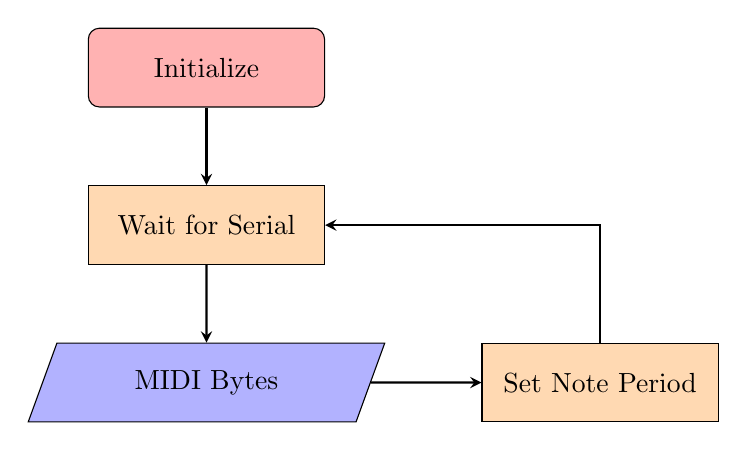
\begin{tikzpicture}[node distance=2cm]

\node (start) [startstop] {Initialize};
\node (process) [process, below of=start] {Wait for Serial};
\node (io) [io, below of=process] {MIDI Bytes};
\node (process1) [process, right of=io, xshift=3cm] {Set Note Period};


\draw [arrow] (start) -- (process);
\draw [arrow] (process) -- (io);
\draw [arrow] (io) -- (process1);
\draw [arrow] (process1) |- (process);

\end{tikzpicture}
\end{center}

This loop is represented in the loop function of the Arduino. This code is continuously waiting for serial data, and then it is parsed. The parsing follows the MIDI file format as discussed in Section \ref{MIDIMESSAGE}. The loop only looks for note on, note off, and channel mode messages.  

\lstinputlisting[language=C, firstline=95,lastline=120]{../src/floppy/floppy.ino}

\section{ISR}

The ISR or interrupt service routine is the routine that gets called every time the interrupt from the timer1 is triggered. The specific code run during this time is the code that does the driving of the floppy drives. The block diagram is as following:

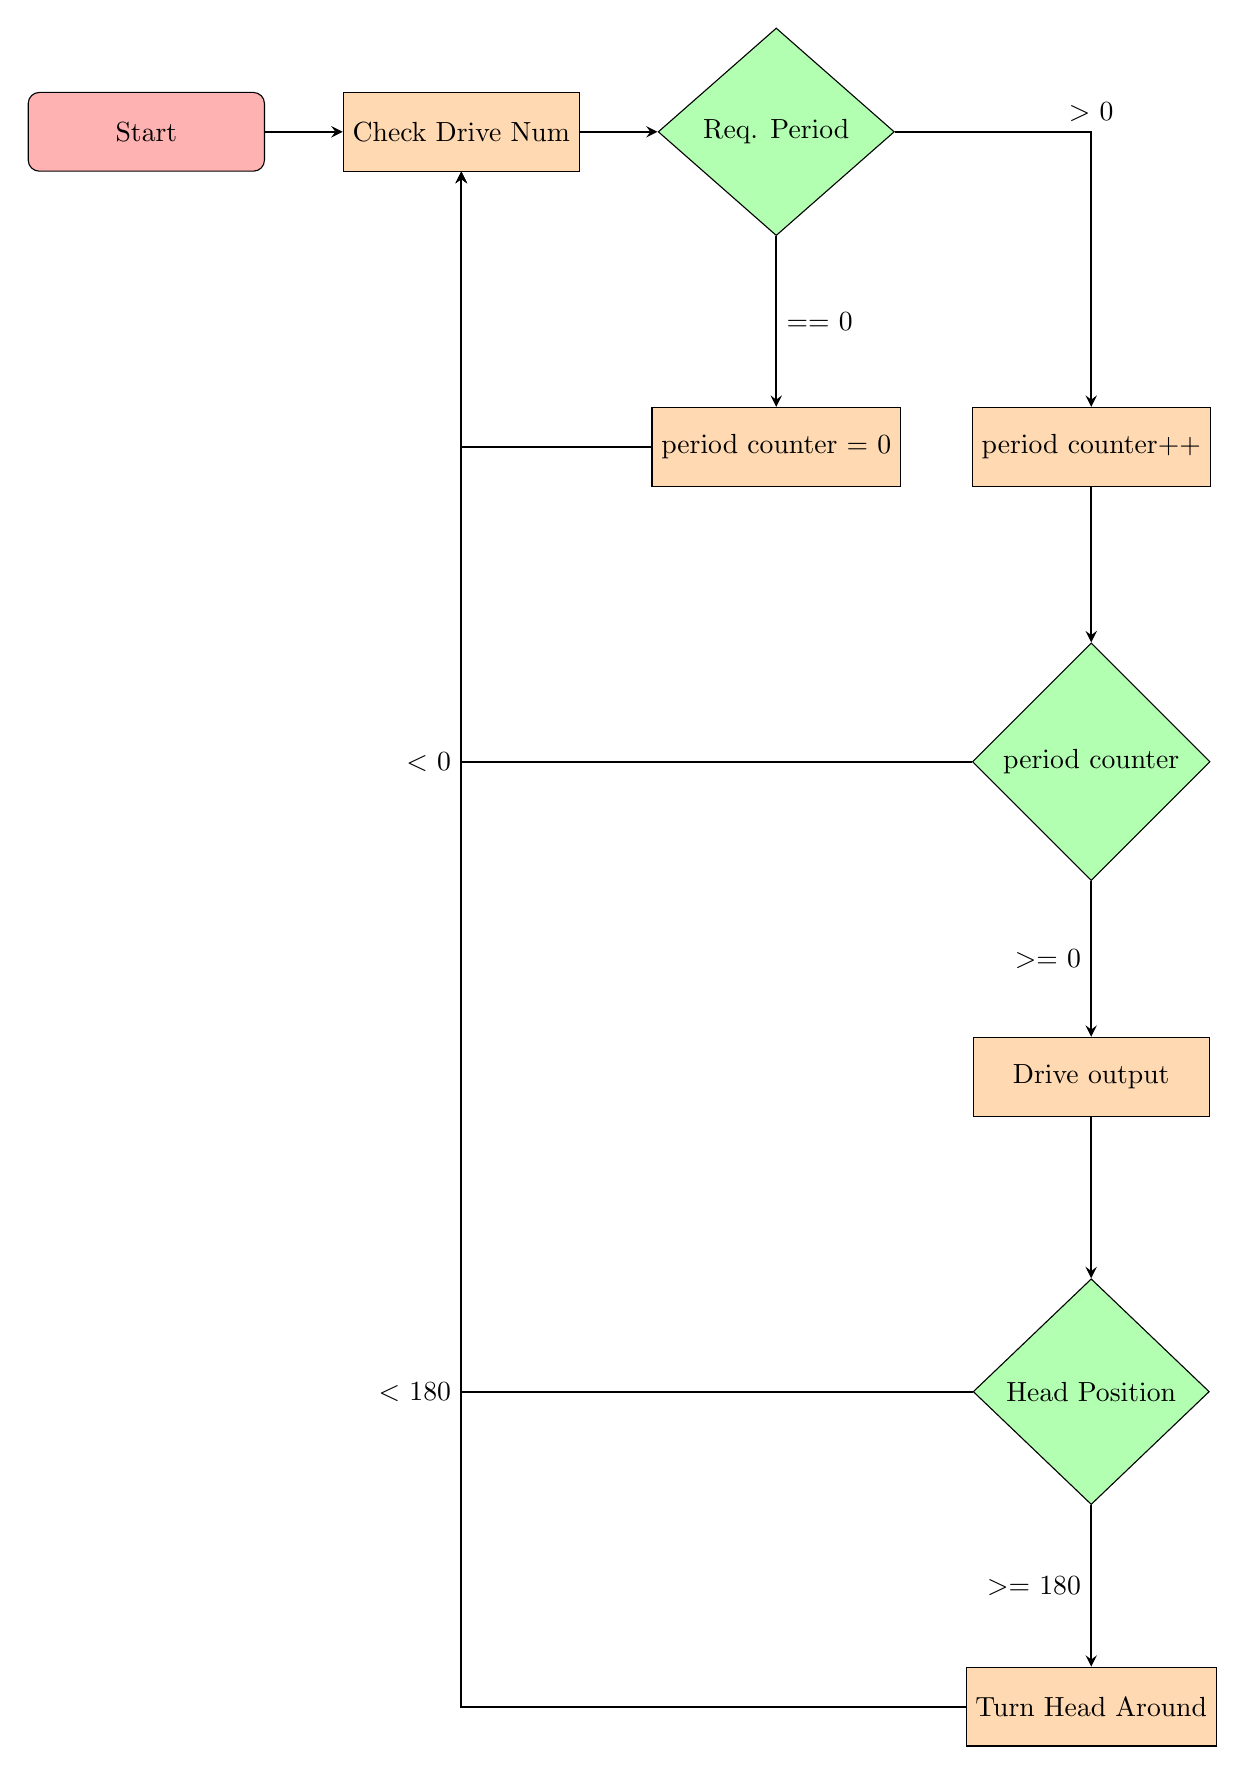
\begin{tikzpicture}[node distance=2cm]

\node (start) [startstop] {Start};
\node (process) [process, right of=start, xshift=2cm] {Check Drive Num};
\node (decision) [decision, right of=process, xshift=2cm] {Req. Period};
\node (process1) [process, below of=decision, yshift=-2cm] {period counter = 0};
\node (process2) [process, right of=process1, xshift=2cm] {period counter++};
\node (decision1) [decision, below of=process2, yshift=-2cm] {period counter};
\node (process3) [process, below of=decision1, yshift=-2cm] {Drive output};
\node (decision2) [decision, below of=process3, yshift=-2cm] {Head Position};
\node (process4) [process, below of=decision2, yshift=-2cm] {Turn Head Around};


\draw [arrow] (start) -- (process);
\draw [arrow] (process) -- (decision);
\draw [arrow] (decision) -- node[anchor=west] {== 0} (process1);
\draw [arrow] (decision) -| node[anchor=south] {$>$ 0} (process2);
\draw [arrow] (process1) -| (process);
\draw [arrow] (process2) -- (decision1);
\draw [arrow] (decision1) -| node[anchor=east] {$<$ 0} (process);
\draw [arrow] (decision1) -- node[anchor=east] {$>$= 0} (process3);
\draw [arrow] (process3) -- (decision2);
\draw [arrow] (decision2) -| node[anchor=east] {$<$ 180} (process);
\draw [arrow] (decision2) --  node[anchor=east] {$>=$ 180}  (process4);
\draw [arrow] (process4) -|(process);

\end{tikzpicture}

\pagebreak
The ISR follows a checklist. It is a for loop that checks each floppy drive's status. It first checks if notePeriod, or the requested period is greater than 0. If it is 0, that means that there is not a note suppose to be playing. Otherwise, it increments the period counter. This period counter is checked if it reached the requested period. If so, it flips the step pin. This action of flipping will cause the read/write head to move. It resets the period counter so that it will start the count again. The head position is kept track as well. This is to make sure that the read/write head does not get stuck at the end. If this variable has reached the maximum value, it will revert the direction by changing the value on the direction pin.


\lstinputlisting[language=C, firstline=121,lastline=156]{../src/floppy/floppy.ino}

\section{SD Card(?)}

\chapter{Conclusion}

\pagebreak

\appendix
\newappendix\label{firstappendix}
\section{Full Arduino Code}

\lstinputlisting[language=C]{../src/floppy/floppy.ino}

\newappendix
\section{Bill of Materials}

\footnotesize{
\captionof{table}{MIDI Message}\label{fig:BOM}
\begin{center}
 \begin{tabular}{|c | c | c | c |} 
 \hline
  \multicolumn{4}{|c|}{BOM} \\ 
 \hline
 ITEM & QUANTITY & COST & LINK \\
 \hline
 Arduino R3 & 1 & \$ 24.95 & \url{https://www.adafruit.com/product/50} \\
 \hline
 Arduino Proto Shield & 1 & \$ 9.95 & \url{https://www.adafruit.com/products/2077} \\
 \hline
 5V 4A Power Supply & 1 & \$ 14.95 & \url{https://www.adafruit.com/products/1466} \\
 \hline
 Breadboard-friendly 2.1mm DC barrel jack & 1 & \$ 0.95 & \url{https://www.adafruit.com/products/373} \\
 \hline
 (2.54mm) Crimp Connector Housing: 2x10-Pin & 2 & \$ 1.99 &  \url{https://www.pololu.com/product/1917} \\
 \hline
  (2.54mm) Crimp Connector Housing: 1x2-Pin & 2 & \$ 0.69 & \url{https://www.pololu.com/product/1901}\\
  \hline
  (2.54mm) Crimp Connector Housing: 2x2-Pin & 2 & \$ 0.59 & \url{https://www.pololu.com/product/1910}\\
 \hline
  (2.54 mm) Female Header: 1x12-Pin & 2 & \$ 0.79 & \url{https://www.pololu.com/product/1030}\\
  \hline
  (2.54 mm) Male Header: 2×40-Pin & 3 & \$ 1.49 & \url{https://www.pololu.com/product/966}\\
  \hline
   Pre-crimped Wires 10-Pack F-F (Black) & 4 & \$ 2.49 & \url{https://www.pololu.com/product/1810}\\
  \hline 
   Pre-crimped Wires 10-Pack F-F (Red) & 2 & \$ 2.49 & \url{https://www.pololu.com/product/1812}\\
  \hline 
   Pre-crimped Wires 10-Pack F-F (Blue) & 1 & \$ 2.49 & \url{https://www.pololu.com/product/1816}\\
  \hline 
   Pre-crimped Wires 10-Pack F-F (Purple) & 1 & \$ 2.49 & \url{https://www.pololu.com/product/1817}\\
  \hline

\end{tabular}
\end{center}
}

\begin{thebibliography}{9}
\bibitem{HairlessMIDI}
\url{http://projectgus.github.io/hairless-midiserial/}
\bibitem{pmidi}
\url{http://alsa.opensrc.org/Pmidi}
\bibitem{ttymidi}
\url{http://www.varal.org/ttymidi/}
\bibitem{VMPK}
\url{http://vmpk.sourceforge.net/}
\bibitem{Music}
\url{https://github.com/coon42/Floppy-Music--midis-/tree/master/midi/finished/MrSolidSnake745}
\bibitem{MIDIStandard}
\url{https://en.wikipedia.org/wiki/MIDI_tuning_standard}
\bibitem{MIDIMessage}
\url{https://www.midi.org/specifications/item/table-1-summary-of-midi-message}
\end{thebibliography}


\end{document}
